\documentclass[a4paper,5pt]{amsbook}
%%%%%%%%%%%%%%%%%%%%%%%%%%%%%%%%%%%%%%%%%%%%%%%%%%%%%%%%%%%%%%%%%%%%%

\usepackage{booktabs}
\usepackage{graphicx}
\usepackage{multicol}
\usepackage{textcomp}
\usepackage{systeme}
\usepackage{amssymb}
\usepackage{amsmath}
\usepackage{subcaption}
\usepackage[inline]{enumitem}
\usepackage[portuguese]{babel}

%%%%%%%%%%%%%%%%%%%%%%%%%%%%%%%%%%%%%%%%%%%%%%%%%%%%%%%%%%%%%%

\newcommand{\sen}{\,\mbox{sen}\,}
\newcommand{\tg}{\,\mbox{tg}\,}
\newcommand{\cosec}{\,\mbox{cosec}\,}
\newcommand{\cotg}{\,\mbox{cotg}\,}
\newcommand{\tr}{\,\mbox{tr}\,}
\newcommand{\ds}{\displaystyle}

%%%%%%%%%%%%%%%%%%%%%%%%%%%%%%%%%%%%%%%%%%%%%%%%%%%%%%%%%%%%%%%%%%%%%%%%

\setlength{\textwidth}{16cm} %\setlength{\topmargin}{-1.3cm}
\setlength{\textheight}{26cm}
\setlength{\leftmargin}{1.2cm} \setlength{\rightmargin}{1.2cm}
\setlength{\oddsidemargin}{0cm}\setlength{\evensidemargin}{0cm}
\setlength{\topmargin}{-1cm}

%%%%%%%%%%%%%%%%%%%%%%%%%%%%%%%%%%%%%%%%%%%%%%%%%%%%%%%%%%%%%%%%%%%%%%%%

% \renewcommand{\baselinestretch}{1.6}
% \renewcommand{\thefootnote}{\fnsymbol{footnote}}
% \renewcommand{\theequation}{\thesection.\arabic{equation}}
% \setlength{\voffset}{-50pt}
% \numberwithin{equation}{chapter}

%%%%%%%%%%%%%%%%%%%%%%%%%%%%%%%%%%%%%%%%%%%%%%%%%%%%%%%%%%%%%%%%%%%%%%%

\begin{document}
\thispagestyle{empty}
\pagestyle{empty}
\begin{minipage}[h]{0.14\textwidth}
	
\includegraphics[scale=0.24]{../../ufgd.png}
\end{minipage}
\begin{minipage}[h]{\textwidth}
\begin{tabular}{c}
{{\bf UNIVERSIDADE FEDERAL DA GRANDE DOURADOS}}\\
{{\bf Geometria --- Lista 3}}\\
{{\bf Prof.\ Adriano Barbosa}}\\
\end{tabular}
\vspace{-0.45cm}
%
\end{minipage}

%------------------------

\vspace{1cm}
%%%%%%%%%%%%%%%%%%%%%%%%%%%%%%%%   formulario  inicio  %%%%%%%%%%%%%%%%%%%%%%%%%%%%%%%%
\begin{enumerate}
    \item Considere um tri\^angulo $ABC$ de lados $a$, $b$ e $c$, conforme a
        figura e seja $r$ o raio do c\'{\i}rculo circunscrito a este tri\^angulo.
        Prove que:
        \[\frac{a}{\sen\hat{A}} = \frac{b}{\sen\hat{B}} = \frac{c}{\sen\hat{C}}
        = 2r\]
        \begin{figure}[!h]
            \centering
            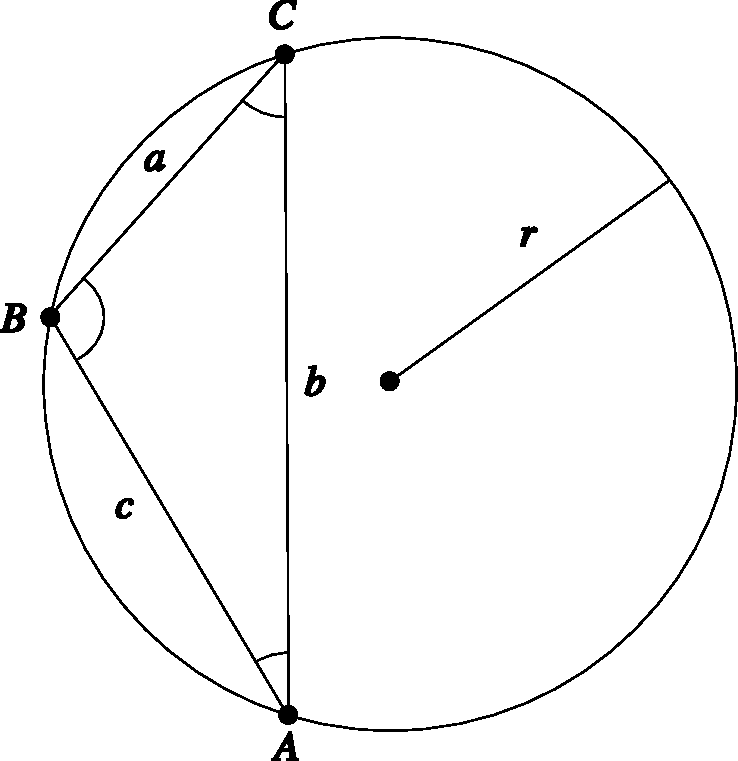
\includegraphics[width=0.3\textwidth]{fig03-1.pdf}
        \end{figure}

    \item Dois tri\^angulos $ABC$ e $BCD$ s\~ao is\'osceles, ret\^angulos em $B$ e
        contidos em planos perpendiculares, conforme a figura. Determine o
        volume do s\'olido $ABCD$ em fun\c{c}\~ao da medida $a$ do segmento $AB$.
        \begin{figure}[!h]
            \centering
            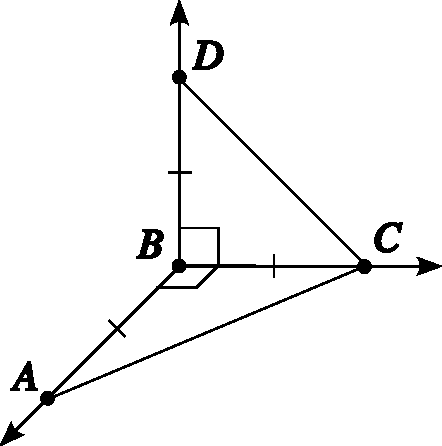
\includegraphics[width=0.3\textwidth]{fig03-2.pdf}
        \end{figure}

    \item Um octaedro retangular est\'a inscrito em um cubo de aresta 1cm de modo
        que seus v\'ertices s\~ao os centros das faces de um cubo. Determine:
        \begin{enumerate}
            \vspace{0.3cm}
            \item A medida da aresta do octaedro.
            \vspace{0.3cm}
            \item O volume do octaedro.
        \end{enumerate}
        \begin{figure}[!h]
            \centering
            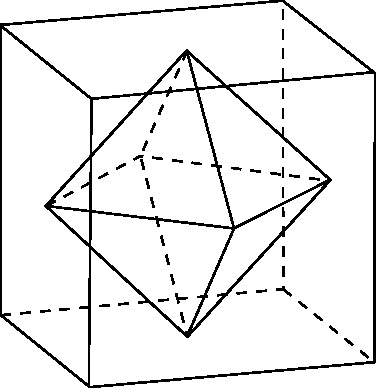
\includegraphics[width=0.3\textwidth]{fig03-3.pdf}
        \end{figure}

    \item Na figura, $AB$ \'e um di\^ametro do c\'{\i}rculo de centro $O$ e raio 5. O
        ponto $C$ pertence ao c\'{\i}rculo, $P$ pertence ao raio $OC$,
        $B\hat{P}C=90^\circ$ e $\overline{OP}=1$. Determine a \'area do tri\^angulo
        $ABC$.
        \begin{figure}[!h]
            \centering
            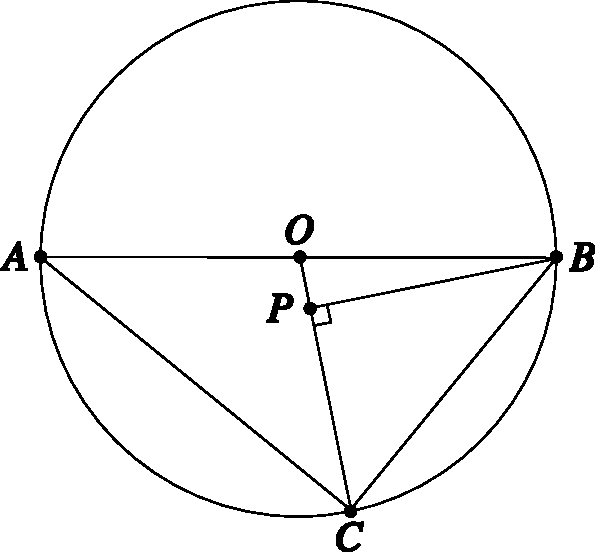
\includegraphics[width=0.3\textwidth]{fig03-4.pdf}
        \end{figure}

    \item As diagonais $AD$ e $CE$ do pent\'agono regular $ABCDE$ de lados de
        medida $a$ se intersectam no ponto $P$. Determine $\overline{AP}$ e
        $\overline{PD}$ em fun\c{c}\~ao de $a$.
        \begin{figure}[!h]
            \centering
            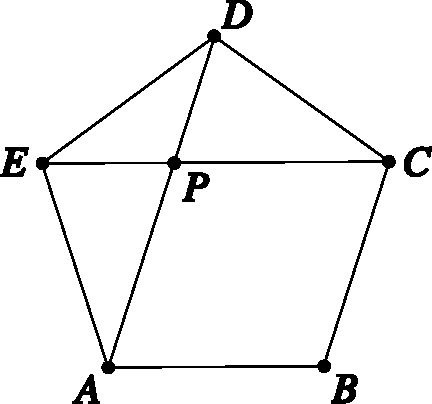
\includegraphics[width=0.3\textwidth]{fig03-5.pdf}
        \end{figure}
\end{enumerate}

\end{document}
